\chapter{Methodology}

\textbf{Author: } 

\section{Stereo Camera}
The challenge of sensing distances to various objects has been solved using stereo vision cameras. Computer stereo vision systems use two horizontally displaced cameras to take two images which then are both processed together to gather the information on the depth of the images. This process can be rather complicated as the distortions (more specifically the barrel distortion and the tangential distortion) of the images have to be undone, before the two images are projected onto a common plane, a disparity map can be created by comparison of the two images and a 3d point cloud can be generated from it. In most robotics applications this point cloud is then filtered in search of some object, which distance was sought-after.

\subsection{Distortion}
Barrel distortion occurs when the lens used by the camera has a higher magnification at the centre of the image than at the sides. This distortion can be visualized as seen in Figure~\ref{pic:methodology_stereoCamera_distortion_barrelDistortion}.

\begin{figure}[h!]
	\centering
	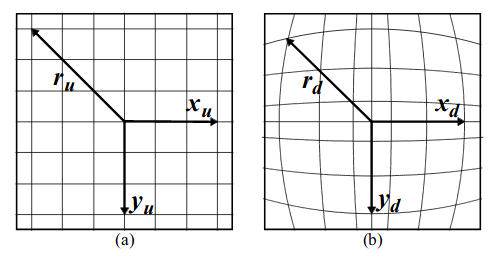
\includegraphics[width=4.5in]{img/methodology_stereoCamera_distortion_barrelDistortion.png}
	\caption{The left shows the original image composed of straight horizontal and vertical lines. On the right image the effect of the barrel distortion can be perceived, which causes the lines to curve toward the outside of the image, causing the lines to appear in a barrel like shape.[TODO: change image to own]}
	\label{pic:methodology_stereoCamera_distortion_barrelDistortion}
\end{figure}

To undo this distortion the pixel values in an undistorted image have to be calculated based on the pixel values in the distorted image.

\begin{equation}
r_u = r_d(1+k r_d^2)
\end{equation}

describes the calculation which computes the distance from the centre in the undistorted image ($r_u$) based on the distance from the centre in the distorted image ($r_d$) and some distortion parameter $k$, which is specific to the lens used. Gribbon et.al. note in their work \footcite{Gribbon_Barrel_Distortion_Correction_Algorithm} that this rarely is an integer value, therefore different equations are proposed:

\begin{equation}
x_d = x_u M(k,r_u^2) \hspace{30pt} y_d = y_u M(k, r_u^2)
\end{equation}

where the magnification factor $M(k,r_u^2)$ is

\begin{equation}
M(k,r_u^2) = \frac{1}{1+k * M(k,r_u^2)^2 * r_u^2}
\end{equation}

Tangential distortion in comparison to barrel distortion displaces points along the tangent of a circle placed at the centre of the image as seen in Figure~\ref{pic:methodology_stereoCamera_distortion_tangentialDistortion}.

\begin{figure}[h!]
	\centering
	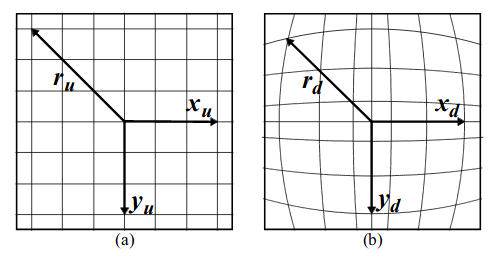
\includegraphics[width=2in]{img/methodology_stereoCamera_distortion_tangentialDistortion.png}
	\caption{A point $P$ is distorted along the tangent $t$ of a circle placed at the middle of the image $C$ with a radius $r$ to a point $P'$. Distortions of this form are called tangential distortions.}
	\label{pic:methodology_stereoCamera_distortion_tangentialDistortion}
\end{figure}

The radius of the circle in Figure~\ref{pic:methodology_stereoCamera_distortion_tangentialDistortion} is dependent on the point $P$. It can be calculated as the length between $P$ and $C$. The length of the vector $PP'$ is not uniform for all points and therefore depends on point $P$.

\subsection{Image Rectification}

\subsection{Disparity Map}

\subsection{3d point cloud}

\subsection{Challenges}
Since many drones used in educational robotics can only carry a limited amount of weight it is not possible to attach a stereo camera to such a robot. Instead the drone has to take the first image, fly to a second position located horizontally next to the first one and take the second image. This process in not as precise as a stereo camera, where the two lenses are always positioned at an exact interval from one another. Therefore the output of this system might not work as reliable. Additionally other factors, such as differences in the two images due to some time passing between the taking of the images can have an effect on the accuracy.

Therefore the authors try to approach this challenge from the machine learning point of view. Neural networks can be taught to work with different changes in the environment and still return results with a superior quality to conventional implementation.

\section{Generating data}
Neural Networks require huge amounts of data to work reliably. Because of the author's limited time frame this test data will be generated with the help of Blender 2.8. Blender is a free program for designing and animating 3D objects, which also supports scripting with python to add or remove objects from a scene. The authors will use this capability to generate the huge amounts of test data needed from the perspectives of the 2 cameras, which point to a specific object in the scene. This enables the authors to use and train a neural network, since shooting the amount of pictures needed by hand would take too long to consider this idea.

\subsection{Blender}
Besides 3D-modelling Blender enables the user to perform various different actions, such as laying out scenes, UV-Editing, shading, animating and rendering. Additionally scenes can be modified by executing Python scripts. Figure~\ref{pic:methodology_generatingData_blender_startscreen} shows the interface of Blender 2.8 with the default file loaded.

\begin{figure}[h!]
	\centering
	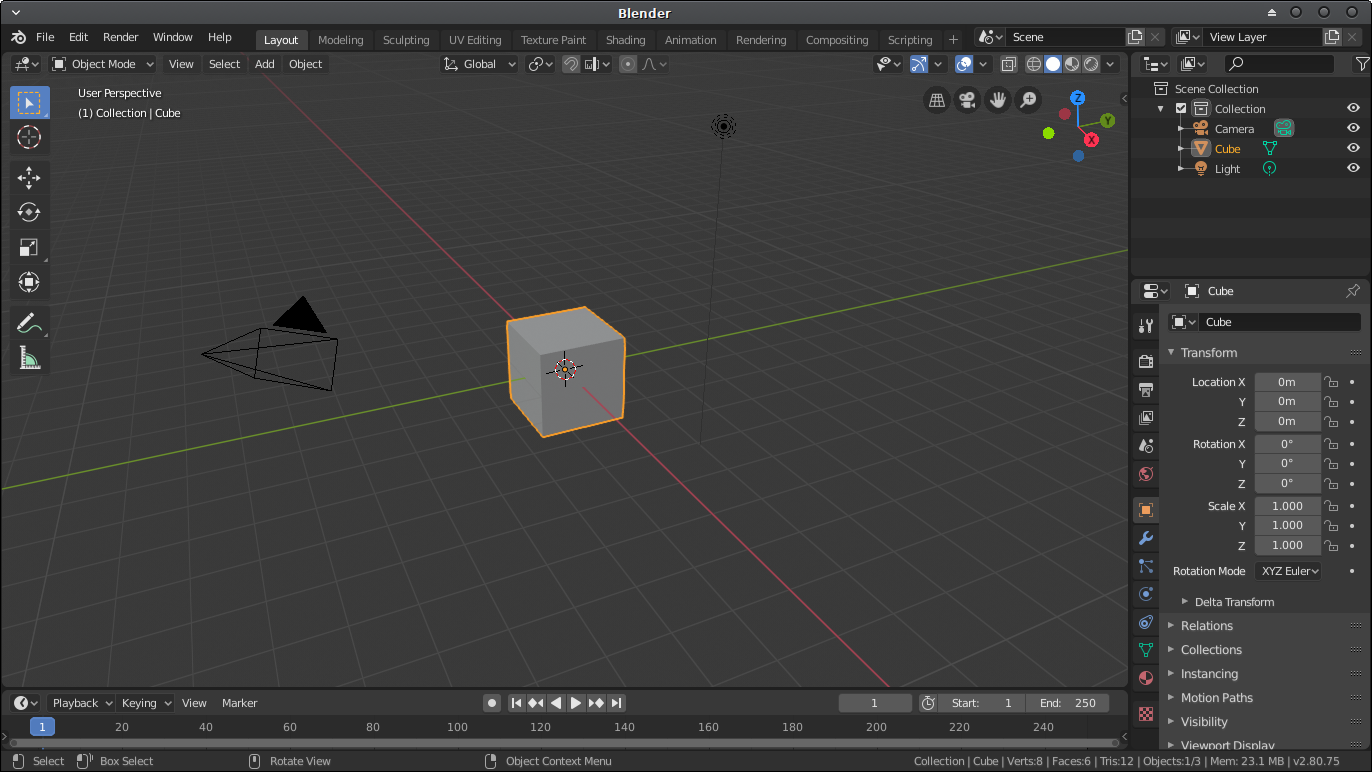
\includegraphics[width=6.5in]{img/methodology_generatingData_blender_startscreen.png}
	\caption{Blender interface after startup. The default scene features a grey cube, a camera (left of the cube) and a light source (black dot and circle positioned on the top right of the cube).}
	\label{pic:methodology_generatingData_blender_startscreen}
\end{figure}

The authors decided to extensively use the scripting function in their work. One example of a Python script, that can be executed in blender is the following code:

\begin{lstlisting}[language=python]
python code
\end{lstlisting}

It modifies ...

\section{Image preprocessing}
After the test images have been rendered with the help of Blender, the authors decided to experiment if manipulating these test images would result in differences of distance perception by the neural network. This manipulation is done with OpenCV in Python3. OpenCV provides a lot of image manipulation tools; for this experiment the authors chose the following methods of image manipulation:

[
schwarz-weiß?
\subsection{Greyscale}
A greyscale image is an image with only one value for the red, green and blue colour channels, resulting in different shades of grey instead of usual colours. This can easily be achieved by the following OpenCV code:

auflösung?
filter?
object detection?
]

\section{Neural Network}
The authors decided to use a software framework called TensorFlow for the first implementation of the neural network. This has the following two advantages: using Tensorflow allows for a low effort proof of concept and it makes testing out different configurations (e.g. number of hidden layers or filters in image preprocessing) of the neural network easier.

After it has been shown that the challenge of detecting the distance to an object can be solved using machine learning, the authors plan on implementing a neural network in C++ on their own. The knowledge gained in the TensorFlow implementation will be used in the C++ implementation, which hopefully will make the work less time consuming.

\section{TensorFlow}
As machine learning has gained popularity in recent years the demand for applicable frameworks grew. One of the most popular is called TensorFlow. It was developed by Google for internal use and was published under the Apache License 2.0 on the \nth{9} of November 2015.

TensorFlow supports APIs for Python, C, C++, Go, Java, JavaScript and Swift.
Due to its popularity third party APIs for C\#, R, Scala, Rust and many more were developed.

Its use cases reach from categorizing handwritten digits to YouTube video recommendations, one of the many applications Google use it for.

Tom Hope et al. describe TensorFlow as a software framework for numerical computations based on dataflow graphs \footcite[page 6]{Hope_Learning_TensorFlow}.

\subsection{Computation graph}
To compute a value using TensorFlow a computation graph has to be constructed. In this graph each node corresponds to an operation, such as subtraction or division. By connecting these nodes via edges the output of one node can be fed as input into another node. One example of such a computation graph can be seen in Figure~\ref{pic:implementation_tensorflow_nodesAndGraphs_computationGraph}.

\begin{figure}[h!]
	\centering
	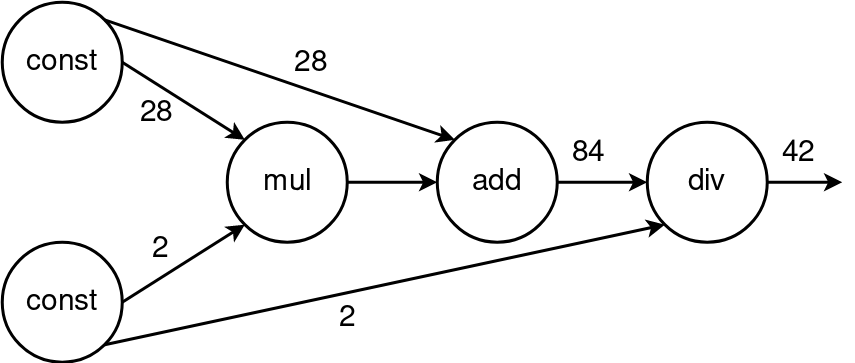
\includegraphics[width=4.5in]{img/implementation_tensorflow_nodesAndGraphs_computationGraph.png}
	\caption{Each node represents an operation, where $const$ stands for a constant value, $add$ for addition, $mul$ for multiplication and $div$ for division. Edges, represented by arrows, connect nodes. The information shared between the nodes is described by the numbers written next to the edges. This computational graph calculates the result of the arithmetic expression $(28 * 2) + 28 / 2$.}
	\label{pic:implementation_tensorflow_nodesAndGraphs_computationGraph}
\end{figure}

The implementation of the computation graph, shown in Figure~\ref{pic:implementation_tensorflow_nodesAndGraphs_computationGraph}, in Python could look as follows:

\begin{lstlisting}[language=python]
import tensorflow as tf

a = tf.constant(28)
b = tf.constant(2)

c = tf.multiply(a, b)
d = tf.add(a, c)
e = tf.divide(d, b)

with tf.Session() as sess:
out = sess.run(e)

print(out)
\end{lstlisting}

The first line specifies that the TensorFlow functionality should be imported. Line 3 and 4 define the two constant values and assigns them the values 28 and 2 respectively. In line 6 to 8 the other nodes of the graph are specified. E.g. in line 6 a new node, named $c$, is created and the output of node $a$ and node $b$ are connected as its input. To perform the calculation described by the graph a new session is created in line 10. Finally the output of the graph (node $e$) is specified in line 11, the result is calculated and printed in line 13.

TensorFlow allows for another way of specifying a graph with these arithmetic operations:

\begin{lstlisting}[language=python]
import tensorflow as tf

a = tf.constant(28)
b = tf.constant(2)

e = (a * b + a) / b

with tf.Session() as sess:
out = sess.run(e)

print(out)
\end{lstlisting}

This code is equivalent to the first one, but uses syntactic sugar to shorten line 6 to 8 in the first code block into line 6. At this point it should be noted that while it might look like it line 6 does not calculate anything. It simply describes how the computational graph should look. The answer (42) is calculated in the session in line 9.

\subsection{Convonutional Neural Networks?}

\subsection{Alternatives to Tensorflow}
[INFO: Abstraction libraries such as Keras and TF-Slim offer simplified  high-level  access  to  the  "LEGO  bricks"  in  the  lower-level  library,  helping  to streamline the construction of the dataflow graphs, training them, and running inference. \footcite[page 7]{Hope_Learning_TensorFlow}]

\begin{center}
	\begin{tabular}{| l | l | l | l | l |}
		\hline
		\bfseries & \bfseries Open Source & \bfseries Actively & \bfseries Parallelization & \bfseries Interface \\
		& & \bfseries developed & & \\
		\hline
		\bfseries TensorFlow & Yes & Yes & Yes & Python, C, C++, \\
		& & & & Go, Java, JavaScript, \\
		& & & & Swift, R, Julia \\
		\hline
		\bfseries Keras & Yes & Yes & Yes & Python \\
		\hline
		\bfseries PyTorch & Yes & Yes & Yes & Python, C++ \\
		\hline
		\bfseries Torch & Yes & No & Yes & Lua, LuaJIT, C, \\
		& & & & C++, OpenGL \\
		\hline
		\bfseries Wolfram & No & Yes & Yes & Wolfram Language \\
		\bfseries Mathematica & & & & \\
		\hline
	\end{tabular}
	\label{tab:implementation_tensorflow_alternativesToTensorflow_comparision}
\end{center}

[+ warum verwenden wir ausgerechnet Tenserflow]

\filbreak
